\documentclass[UTF8]{article}
\usepackage{ctex}
\usepackage{amsmath}
\usepackage{graphicx}
\usepackage{listings}
\usepackage{color}
\usepackage{geometry}
\usepackage{caption}
\usepackage[dvipsnames]{xcolor} % 更全的色系
\usepackage{listings} % 排代码用的宏包
\usepackage{svg}
\usepackage{subcaption}
\usepackage{hyperref}
% Page layout
\geometry{a4paper, margin=1in}

% Title and Author
\title{Chapter 5 Image restoration and Reconstruction}
\author{李想 \quad P12214061}

\begin{document}

\maketitle
\section{问题一}
在傅里叶变换中,周期性噪声在对应于周期干扰的频率处显示为集中突发的能量。方法是用一个选择性滤波器
来分离噪声。简单的周期噪声,在空域中表现为一个个的条纹(摩尔纹),我们可以用陷波滤波器来去除它。

观察原始图像图\ref{fig:original_image},我们能够发现图\ref{fig:original_image}中存在周期性的、近似水平的噪声模式。
\begin{figure}[htbp]
    \centering
    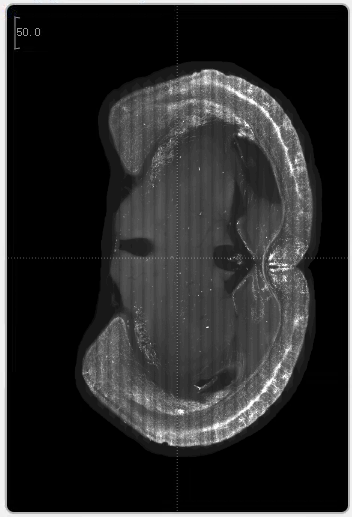
\includegraphics[width=0.4\textwidth,angle=90]{fMOST/fMOST鼠脑图1.png}
    \caption{原始图像}
    \label{fig:original_image}
\end{figure}
对图\ref{fig:original_image}进行傅里叶变换,得到频域的幅值谱和相位谱,如图\ref{fig:fft}所示。
在频域图像中,我们并没有看到一些突出的频率分量。

\begin{figure}[htbp]
    \centering
    \begin{subfigure}{0.4\textwidth}
      \centering
      \includesvg[width=0.6\textwidth]{img/amp.svg}
      \caption{幅值谱}
      \label{fig:amp} % 规范命名
    \end{subfigure}
    % \hfill
    \begin{subfigure}{0.4\textwidth}
      \centering
      \includesvg[width=0.6\textwidth]{img/ph.svg}
      \caption{相位谱}
      \label{fig:phase} % 规范命名
    \end{subfigure}
    \caption{原始图像的傅里叶变换}
    \label{fig:fft} % 主图标签保持原样
\end{figure}
观察周期性条纹,我们发现条纹近似水平,我们认为其在频率域中的贡献集中在DFT的纵轴上。
然而,这一噪声不足以在纵轴上产生清晰的模式。此时采用的方法是使用沿纵轴延申的一个窄
矩形陷波滤波器,来消除沿纵轴分布的所有干扰分量。在接近原点的位置不进行滤波,以避免
消除直流项和低频分量。图\ref{fig:filter}显示了我们所用的滤波器函数。
\begin{figure}[htbp]
    \centering
    \begin{subfigure}{0.4\textwidth}
      \centering
      \includesvg[width=0.8\textwidth]{img/filter.svg}
      \caption{陷波带阻滤波器}
      \label{fig:filter} % 规范命名
    \end{subfigure}
    % \hfill
    \begin{subfigure}{0.4\textwidth}
      \centering
      \includesvg[width=0.8\textwidth]{img/filter2.svg}
      \caption{陷波带通滤波器}
      \label{fig:filter2}% 规范命名
    \end{subfigure}
    \caption{滤波器函数}
    \label{fig:filters} % 主图标签保持原样
\end{figure}

图\ref{fig:output}显示了滤波后的结果。大部分周期性条纹被消除或明显减弱。
为得到噪声的的模式图像,我们首先将带阻滤波器转换为带通滤波器,如图\ref{fig:filter2}所示。
然后将其应用于原始图像。图\ref{fig:output2}显示了滤波器滤出的噪声模式,为一些列周期性条纹。
\begin{figure}[htbp]
    \centering
    \begin{subfigure}{0.45\textwidth}
      \centering
      \includesvg[width=\textwidth]{img/output.svg}
      \caption{滤波后的图像}
      \label{fig:output}
    \end{subfigure}
    % \hfill
    \begin{subfigure}{0.45\textwidth}
      \centering
      \includesvg[width=\textwidth]{img/噪声模式.svg}
      \caption{陷波滤波从图\ref{fig:original_image}中提取出的噪声模式}
      \label{fig:output2}
    \end{subfigure}
    \caption{陷波滤波的输出}
    \label{fig:outputs} % 主图标签保持原样
\end{figure}
% \begin{figure}[htbp]
%     \centering
%     \includesvg[width=0.8\textwidth]{img/output.svg}
%     \caption{滤波后的图像}
%     \label{fig:output}
% \end{figure}
% \begin{figure}[htbp]
%     \centering
%     \includesvg[width=0.8\textwidth]{img/噪声模式.svg}
%     \caption{陷波滤波从图\ref{fig:original_image}中提取出的噪声模式}
%     \label{fig:output}
% \end{figure}
\section{问题二}

    运动模糊的图像可以用逆滤波和维纳滤波来恢复。
    逆滤波是基于图像的频域表示,假设模糊核已知。
    维纳滤波则是基于图像的统计特性,假设噪声和模糊核已知。

\subsection{模糊核推导}
    下面匀速线性运动模糊核:
    % -------------- start of snippet ----------------

    假设图像 $f(x,y)$ 做平面运动,$x_0(t)$ 和 $y_0(t)$ 分别是运动在 x 方向和 y 方向上的时变分量。记录介质(如胶片或数字存储器)上任何一点的总曝光量,是成像系统快门打开期间的瞬时曝光量的积分。
假设快门开关是瞬间发生的,并且光学成像过程是完美的,这可让我们隔离由图像运动产生的影响。于是,若 $T$ 是曝光的持续时间,则有
\begin{equation}
 g(x,y) = \int_0^T f(x - x_0(t), y - y_0(t)] dt 
 \label{equation1}
\end{equation}
式中,$g(x,y)$ 是被模糊的图像。
这个表达式的连续傅里叶变换为
\begin{equation}
 G(u,v) = \int_{-\infty}^{\infty} \int_{-\infty}^{\infty} g(x,y) e^{-j2\pi(ux+vy)} dx dy 
 \label{equation2}
\end{equation}
将式 (\ref{equation1} )代入式 (\ref{equation2}) 得
\begin{equation}
 G(u,v) = \int_{-\infty}^{\infty} \int_{-\infty}^{\infty} \left[ \int_0^T f(x-x_0(t), y-y_0(t)) dt \right] e^{-j2\pi(ux+vy)} dx dy 
 \label{equation3}
\end{equation}
颠倒积分的顺序得
\begin{equation}
     G(u,v) = \int_0^T \left[ \int_{-\infty}^{\infty} \int_{-\infty}^{\infty} f(x-x_0(t), y-y_0(t)) e^{-j2\pi(ux+vy)} dx dy \right] dt 
\label{equation4}
\end{equation}
方括号内的积分项是位移函数 $f[x-x_0(t), y-y_0(t)]$ 的傅里叶变换。
\begin{equation}
 G(u,v) = \int_0^T F(u,v) e^{-j2\pi[ux_0(t)+vy_0(t)]} dt = F(u,v) \int_0^T e^{-j2\pi[ux_0(t)+vy_0(t)]} dt  
\label{equation5}
\end{equation}
定义
\begin{equation}
 H(u,v) = \int_0^T e^{-j2\pi[ux_0(t)+vy_0(t)]} dt  
\label{equation6}
\end{equation}
可将式(\ref{equation5}) 表示为我们熟悉的形式:
\begin{equation}
 G(u,v) = H(u,v) F(u,v)
\label{equation7}
\end{equation}
若运动分量 $x_0(t)$ 和 $y_0(t)$ 是已知的,则可直接由式(\ref{equation6})得到传递函数 $H(u,v)$。如说明的那样,假设图像只在 x 方向 [即 $y_0(t)=0$] 做速率为 $x_0(t)=at/T$ 的匀速直线运动。当 $t=T$ 时,图像移动的总距离为 $a$。令 $y_0(t)=0$,由式(\ref{equation6})可得
\begin{equation}
    H(u,v) = \int_0^T e^{-j2\pi u x_0(t)} dt = \int_0^T e^{-j2\pi u at/T} dt = \frac{T}{\pi u a} \sin(\pi u a) e^{-j\pi u a} 
    \label{equation8}
\end{equation}
若允许图像同时在 y 方向做速率为 $y_0(t)=bt/T$ 的匀速直线运动,则退化函数变为
\begin{equation}
    \boxed{
    H(u,v) = \frac{T}{\pi(ua+vb)} \sin[\pi(ua+vb)] e^{-j\pi(ua+vb)} 
    }
\label{euation9}
\end{equation}
为生成一个大小为 $M \times N$ 的离散滤波器传递函数,我们可在 $u=0,1,2,...,M-1$ 和 $v=0,1,2,...,N-1$ 处对上式取样。

    % -------------- end of snippet ----------------
\subsection{逆滤波}
    逆滤波是基于图像的频域表示,假设模糊核已知。
    在没有噪声的情况下,估计图像为
    \begin{equation}
        \hat{F}(u,v) = \frac{G(u,v)}{H(u,v)}
        \label{equation10}
    \end{equation}
    逆滤波器的缺点是对噪声非常敏感。在有噪声的情况下
    \begin{equation}
        G(u,v) = H(u,v)F(u,v) + N(u,v)
        \label{equation11}
    \end{equation}
    两边同除$H(u,v)$得到估计图像
    \begin{equation}
    \hat{F}(u,v) = F(u,v) + \frac{N(u,v)}{H(u,v)}
    \label{equation12}
    \end{equation} 
取$H(u,v)$为模糊核,令$T = 1$,$a = 0.1$,$b = 0.1$,将模糊核作用于原始图像图\ref{fig:original_img2},
得到模糊后的图像图\ref{fig:blurred_img}。
\begin{figure}[htbp]
    \centering
    \begin{subfigure}{0.45\textwidth}
      \centering
      \includesvg[width=\textwidth]{img/original2.svg}
      \caption{原始图像}
      \label{fig:original_img2}
    \end{subfigure}
    % \hfill
    \begin{subfigure}{0.45\textwidth}
      \centering
      \includesvg[width=\textwidth]{img/blurred.svg}
      \caption{运动模糊后的图像}
      \label{fig:blurred_img}
    \end{subfigure}
    \caption{陷波滤波的输出}
    \label{fig:inputs} 
\end{figure}

在无噪声的情况下,使用逆滤波器恢复图像。图\ref{fig:inverse_filter}显示了恢复后的图像。
\begin{figure}[htbp]
    \centering
    \includesvg[width=0.5\textwidth]{img/recover.svg}
    \caption{逆滤波恢复后的图像}
    \label{fig:inverse_filter}
\end{figure}
观察发现,恢复后的图像几乎与原始图像一致。运动造成的模糊已被去除。

对运动模糊图像的频谱中,加入均值为0,方差为1的高斯噪声,再次使用
逆滤波器,得到恢复后的图像图\ref{fig:inverse_filter2},在图\ref{fig:inverse_filter2}中
原始图像完全不可见,这是因为逆滤波器对噪声敏感,在逆滤波器值较小的情况下噪声被放大,
噪声成为了图像的主导项。为了解决这一为题,我们将逆滤波器的频率限制在原点附近,经过不断调试离原点的
距离,最终得到限制频率的逆滤波恢复的图像图\ref{fig:inverse_filter3}。观察到,噪声已不再是图像的主导项,
可以看到略微模糊的原始图像。
\begin{figure}[htbp]
    \centering
    \begin{subfigure}{0.45\textwidth}
      \centering
      \includesvg[width=\textwidth]{img/filted2.svg}
      \caption{有噪声时逆滤波恢复的图像}
      \label{fig:inverse_filter2}
    \end{subfigure}
    % \hfill
    \begin{subfigure}{0.45\textwidth}
      \centering
      \includesvg[width=\textwidth]{img/filted3.svg}
      \caption{限制频率的逆滤波恢复的图像}
      \label{fig:inverse_filter3} 
    \end{subfigure}
    \caption{有噪声的情况}
    \label{fig:inputs} 
\end{figure}
\subsection{维纳滤波}
维纳滤波则是基于图像的统计特性,假设噪声和模糊核已知。
误差函数最小值在频域中可表示为
\begin{equation}
    \hat{F} = [\frac{1}{H(u,v)}\frac{|H(u,v)|^2}{|H(u,v)|^2+ \frac{S_N(u,v)}{S_F(u,v)}}]G(u,v)
    \label{equation13}
\end{equation}
将模糊核带入式(\ref{equation13}),得到复原图像$\hat{F}(u,v)$,如图\ref{fig:wiener_filter}所示。
\begin{figure}[htbp]
    \centering
    \includesvg[width=0.7\textwidth]{img/wiener.svg}
    \caption{维纳滤波恢复后的图像}
    \label{fig:wiener_filter}
\end{figure}
维纳滤波没有出现噪声被放大的现象,恢复后的图像比逆滤波恢复的图像更清晰。
\end{document}
